\documentclass[11pt,a4paper]{book}
\usepackage[brazilian]{babel}
\usepackage[utf8]{inputenc}
\usepackage[T1]{fontenc}
\usepackage[inline]{enumitem}
\usepackage{xcolor}
\usepackage{listings}
\usepackage{graphicx}
\usepackage{multicol}
\usepackage{amsmath}

\definecolor{mGreen}{rgb}{0,0.6,0}
\definecolor{mGray}{rgb}{0.5,0.5,0.5}
\definecolor{mPurple}{rgb}{0.58,0,0.82}
\definecolor{backgroundColour}{rgb}{0.95,0.95,0.92}

\lstdefinestyle{CStyle}{
    backgroundcolor=\color{backgroundColour},   
    commentstyle=\color{mGreen},
    keywordstyle=\textbf{\color{black}},
    numberstyle=\tiny\color{mGray},
    stringstyle=\color{mPurple},
    basicstyle=\footnotesize,
    breakatwhitespace=false,         
    breaklines=true,                 
    captionpos=b,                    
    keepspaces=true,                 
    numbers=left,                    
    numbersep=5pt,                  
    showspaces=false,                
    showstringspaces=false,
    showtabs=false,                  
    tabsize=2,
    frame=single,
    escapeinside={(*}{*)},
    language=C
}

\makeatletter
% This command ignores the optional argument for itemize and enumerate lists
\newcommand{\inlineitem}[1][]{%
\ifnum\enit@type=\tw@
    {\descriptionlabel{#1}}
  \hspace{\labelsep}
\else
  \ifnum\enit@type=\z@
       \refstepcounter{\@listctr}\fi
    \quad\@itemlabel\hspace{\labelsep}
\fi}
\makeatother

\newcommand{\onestaritem}{\refstepcounter{enumi}\item[$*$\theenumi.]}
\newcommand{\twostaritem}{\refstepcounter{enumi}\item[$**$\theenumi.]}

\title{Lista 1: Fundamentos Estatísticos para Ciência dos Dados}
\author{Ricardo Pagoto Marinho}

\begin{document}
\maketitle
	\begin{enumerate}
		\item
		\begin{itemize}
			\item Enumerável
			\item Enumerável
			\item Enumerável
			\item Enumerável
			\item Não enumerável
			\item Não enumerável
			\item Não enumerável
		\end{itemize}
		\item
		\begin{itemize}
			\item Verdadeiro
			\item Falso
			\item Verdadeiro
			\item Verdadeiro
			\item Falso
			\item Falso
			\item Falso
			\item Falso
			\item Verdadeiro
		\end{itemize}
		\item
		\begin{itemize}
			\item Um círculo de raio 1 centrado na origem
			\item Um círculo de raio 2 centrado na origem
			\item Um círculo de raio 1 centrado no ponto (2,-1)
			\item Uma elipse com menor raio 1 e maior raio 2 centrada em (2,-1)
		\end{itemize}
		\item
		\begin{itemize}
			\item
			\begin{figure}[b]
				\centering
				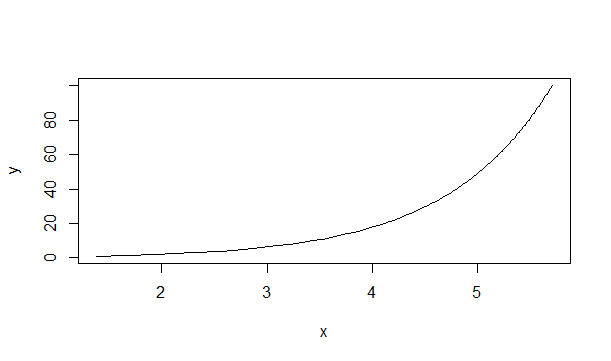
\includegraphics[height=5cm]{4-1.png}
				\caption{log(3x+1)}
			\end{figure}
			\begin{figure}[t]
				\centering
				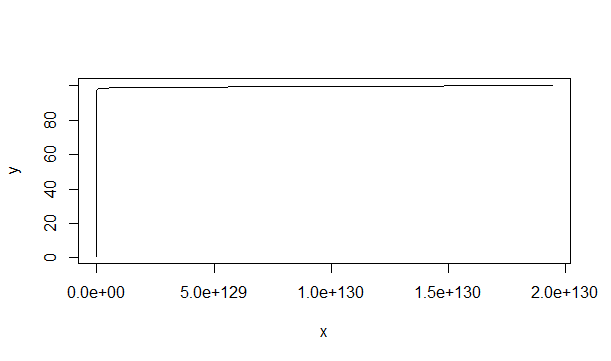
\includegraphics[height=5cm]{4-2.png}
				\caption{exp(3x)}
			\end{figure}
			Domínio: $x>\frac{-1}{3}$
			\item $f(x)=log(3x+1)\\
			f(x)=h(g(x)) \rightarrow h(x)=log(x) g(x)=3x+1\\
			h'(x)=\frac{1}{x}\\
			g'(x)=3\\
			\\
			f'(x)=h'(g(x))g'(x) \rightarrow \frac{3}{3x+1}\\
			\\
			\\
			f(x)=e^{3x} \rightarrow h(x)=e^{x} g(x)=3x\\
			h'(x)=e^{x}\\
			g'(x)=3\\
			\\
			f'(x)=3e^{3x} $
			\item As igualdades válidas são:
			\begin{itemize}
				\item $log(xy)=log(x) + log(y)$
				\item $e^{x+y}=e^{x}+e^{y}$
				\item $log(\frac{x}{y})=log(x)-log(y)$
				\item $e^{xy}=e^{x^{y}}$
			\end{itemize}
		\end{itemize}
		\newpage
		\item Espera-se que o valor da derivada sempre aumente nesse intervalo e será máxima próximo ao zero.
		\begin{figure}[t]
			\centering
			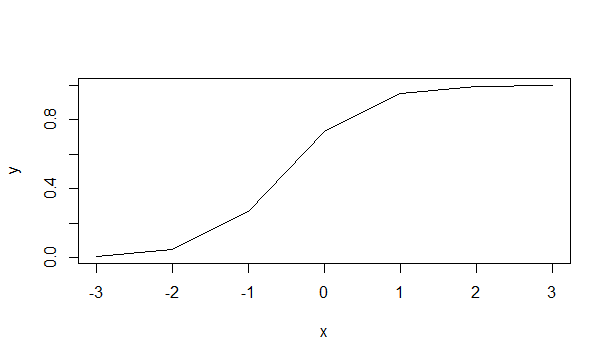
\includegraphics[height=5cm]{5.png}
			\caption{$f(x)=\frac{1}{1+e^{-1-2x}}$}
		\end{figure}
	\end{enumerate}
\end{document}